\chapter{Problem Statement}
\label{chap:ps}
\chaptermark{Problem Statement}

This chapter sets out the problem the project addresses. It describes how Guarantee of Payment requests were handled before the system was built, what that process cost the hospital, which part of it this thesis is concerned with, and what the problem amounts to when stated in short.

\section{Background of the Problem}
\label{sec:ps-background}

A Guarantee of Payment request is assembled from parts held by different people. The patient's identity and insurance details sit with the front desk, the clinical description comes from the surgeon, a separate assessment comes from the anaesthetist, and Finance builds the itemised cost from the hospital's own pricing. Each insurer sets its own form and required fields, so the same case may be presented differently depending on who is being asked to pay.

At Intercare Hospital this was done on paper, and the paper travelled. The surgeon and anaesthetist completed their parts and handed the file to the Surgical Coordinator, who checked it for missing information. Where something was missing, the Coordinator went back to the doctor concerned, who either supplied it themselves or gave permission for the Coordinator to enter it on their behalf. Once complete, the file went to Finance for costing, returned to the Coordinator for the patient's acknowledgement, and if the patient agreed went back to Finance to be sent to the insurer. If the patient declined, the case ended there.

The paper file was the control. Only the person holding it could act in that case. Nothing moved forward unless someone carried it, and an incomplete case went back to the doctor. The order of the work, the point at which each group's part ended, and the separation between the clinical and financial sides were all carried by the movement of that paper. None of it was written down as a rule, because none of it needed to be.

Automating this is not just moving the same process onto a screen. Once the file becomes a database record, everyone can reach it at any time, and the sequence the paper enforced no longer exists.

The new system removes the Coordinator as a required stop. The doctors now pass the case to Finance directly. The Coordinator now only watches progress; editing another role's part of a case is no longer something the Coordinator does. This was not the original plan. Early in the work, the Coordinator kept a narrow edit right carried over directly from paper: the ability to adjust a case's pricing after Finance had verified it, on the understanding that the change had been agreed by phone or in person first, with only the audit log to show who made it. The system had no way to check that the conversation actually happened, so the edit was allowed and simply recorded. That exception was closed before the work finished. The Coordinator's editing rights were narrowed to their own scope only, case priority and response-time targets, and the trust-based allowance was removed rather than kept.

\begin{figure}[H]
  \centering
  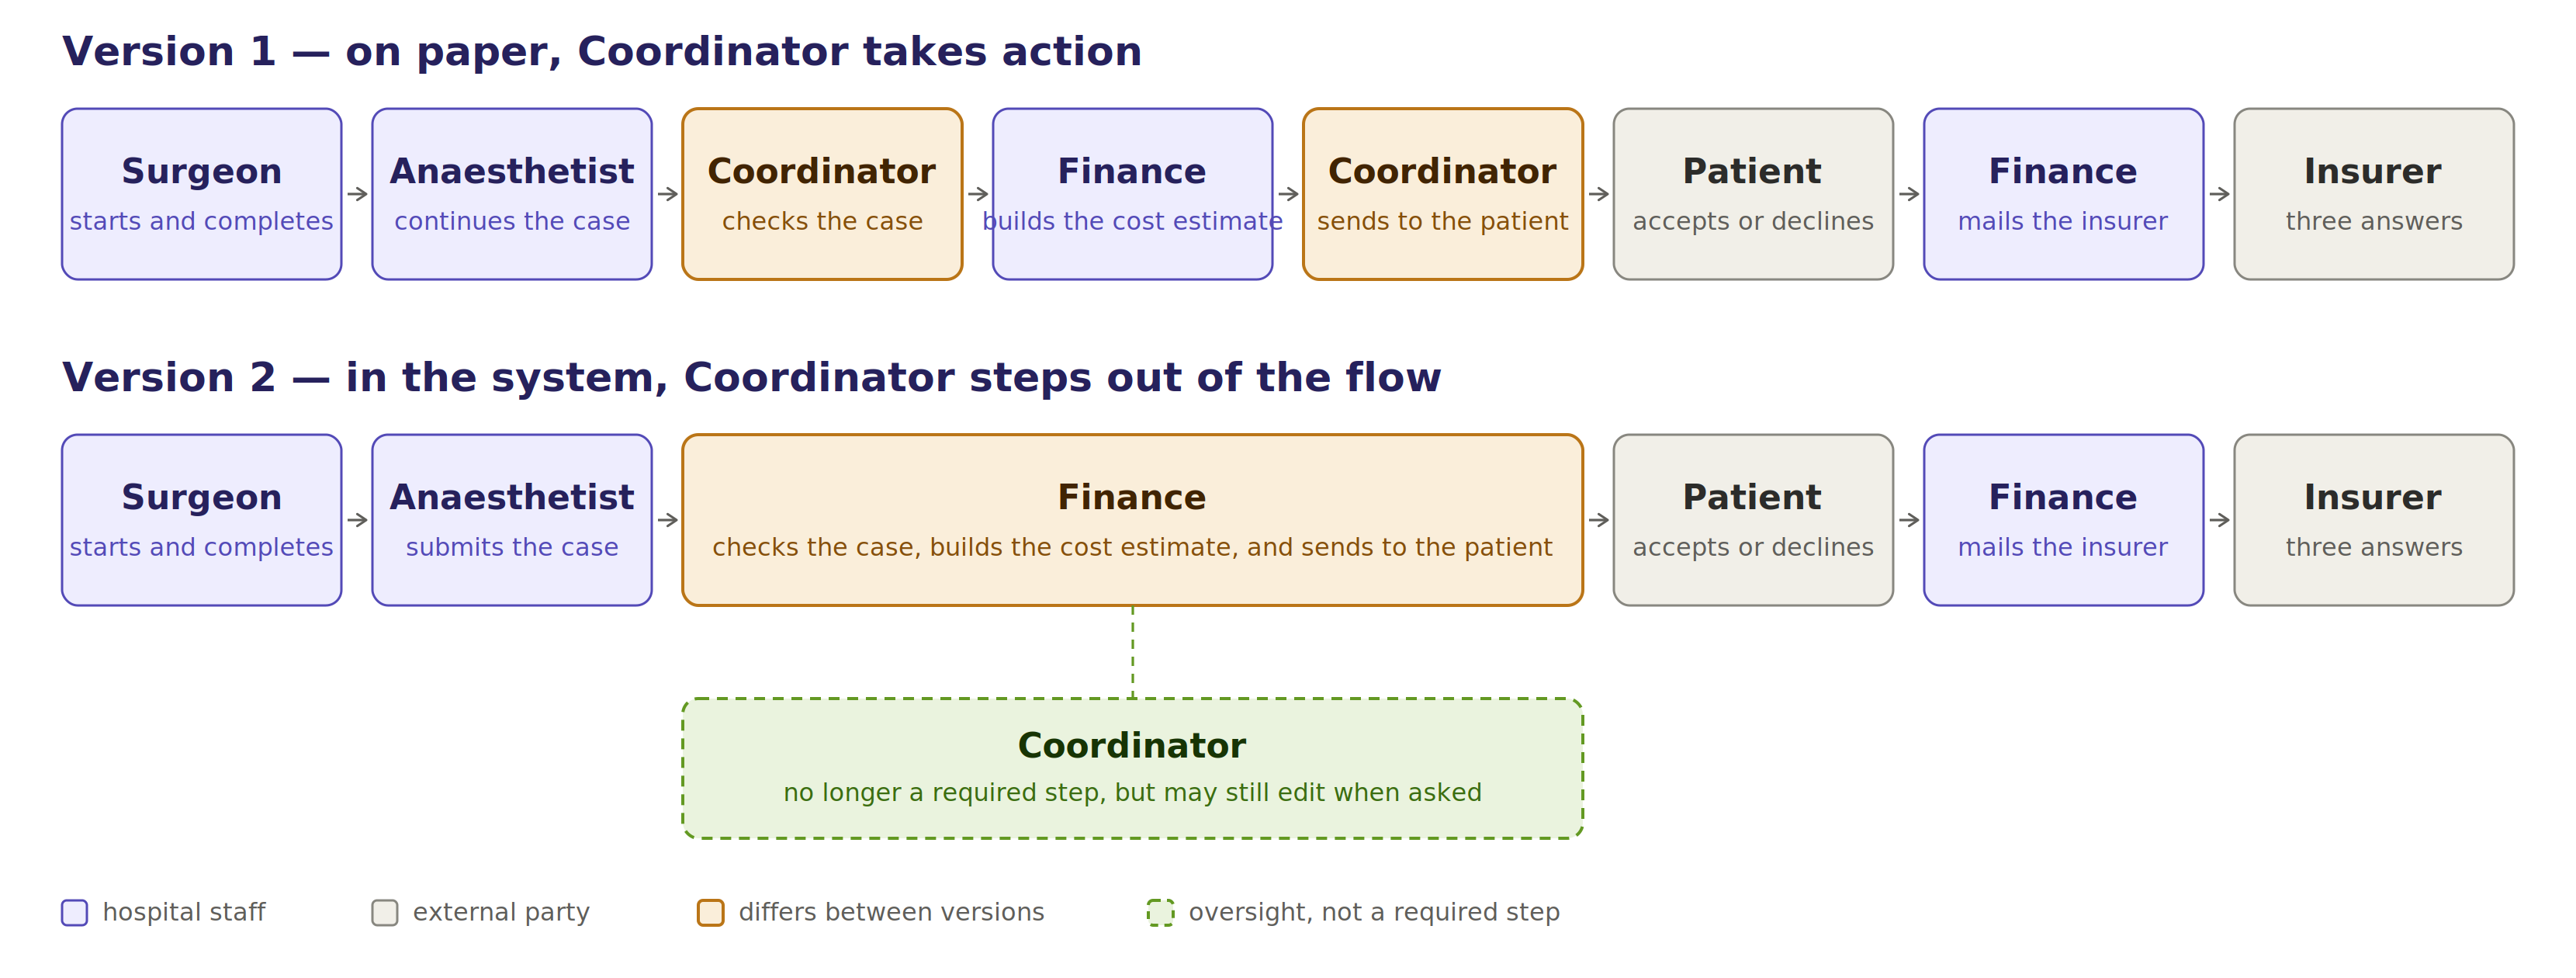
\includegraphics[width=\textwidth]{figs/Figure1-GOP-Process-Flow-Comparison.png}
  \caption{The GOP process on paper compared with the process in the system. Amber marks where the two differ. A patient who declines ends the case; where the insurer asks for changes, Finance revises the request and sends it again.}
  \label{fig:process-comparison}
\end{figure}

On paper, the Coordinator had to walk over and ask before changing a doctor's form. In software, nothing physical stops anyone. So each rule the paper enforced had to become one of two things. Most rules the code blocks outright: the surgeon and anaesthetist can no longer edit a case once it reaches Finance, and the system refuses the change. One rule briefly took the other path, allowed without a check and only logged, trusting that the real-world conversation had happened. That was the Coordinator's pricing edit described above, and it is the only example of that pattern found anywhere in the system. It did not stay that way for long: by the time this work finished, it had been closed and folded into the first kind of rule instead, so every rule the paper enforced is now enforced by code, with no trust-based exception left standing.

\section{Impact of the Problem}
\label{sec:ps-impact}

The manual process cost staff time. Preparing one request meant collecting information that already existed elsewhere. Staff walked between departments to get it, then typed the same patient details more than once as the file moved. A request passed through four departments before it left the hospital, and each hand-off waited on someone being free to receive it.

The clearest case was the handover to Finance. The surgeon and anaesthetist wrote their parts by hand, and Finance then re-entered all of it digitally, because both the patient consent form and the insurer's request had to be produced as documents. With each insurer setting its own format, the same handwritten case could be typed out in more than one layout.

The process also depended on people who are hard to reach. Finance and the Coordinator could not move a case forward until the surgeon and anaesthetist had entered their parts, and staff report that those parts were sometimes forgotten or supplied late. Chasing a doctor who is in theatre or between patients is not quick, so a case could sit waiting on one missing figure.

Order was also difficult to keep. With cases held as paper files, there was nothing to show which had been waiting longest or which needed attention first. Staff report that a case opened early could finish last, and that an emergency case could be delayed simply because the file was hard to find among the others. Nothing about a stack of paper tells you what is urgent.

Repetition also costs accuracy. Details typed a second or third time can be typed differently, a date entered as the fourth month rather than the third, for instance. The information the doctors supplied was correct; the copying was where it went wrong. A mismatch between the patient record, the clinical description and the cost is the kind of error an insurer returns rather than resolves. And because each insurer sets its own form, a missing field found late meant the request came back and the work was done again.

The paper carried its own record. The file showed who the doctors were, who handed it on, and when. That record existed as a by-product of being paper: a signature had to be written, a date entered, and a correction crossed out in view of whoever held the file next. Software keeps none of that by itself. A database shows the current value of a field, not who set it or what it was before. The record has to be built deliberately, or there is none.

\section{Scope of the Problem}
\label{sec:ps-scope}

Not all of the problems described above are addressed here. The security work covers signing in, what each user may do, how their actions are recorded, and the security of the software the system runs on. It also covers the administration screens themselves: the interface for enabling and disabling accounts, and the view onto the audit trail. The application logic, the integration with the hospital information system, and the database design were the work of my teammates, and appear in this thesis only where a security decision depends on them.

Because the system is not internet-facing, this phase focused primarily on authenticated internal users, compromised internal accounts, and misuse of legitimate access, while recognising that external compromise could still occur indirectly through the hospital network, for instance through a stolen credential, a compromised endpoint, or lateral movement from elsewhere on the network. Two checks were outstanding at the time this scope was set: a penetration test by the hospital's IT Security Division, and a review of the container settings against the Center for Internet Security (CIS) Docker Benchmark. The first has since been carried out, by Canadia Bank (IT security department) together with the hospital's IT Security Division. The second, the container review, has also since been carried out by Canadia Bank (IT security department), though not confirmed as following the CIS Docker Benchmark specifically. Going live also required a signed non-disclosure agreement, hospital approval, and privacy safeguards, all agreed at the start of the project.

\section{Summary of the Problem}
\label{sec:ps-summary}

The manual Guarantee of Payment process was slow, repetitive and open to error. It did keep a record of who did what, but only because the paper carried signatures, dates and visible corrections.

Automating it removes the costs. It also removes two things that came free with the paper. The first is the physical route that quietly enforced the order of the work: who could act on a case, at what point their part ended, and where the clinical side stopped and the financial side began. The second is the record itself.

Software will not make people work in order, and it will not keep a history. You have to build both. Every rule must be written into the code. Every action must be saved on purpose. On paper, someone nearby might spot a mistake. In software, no one is nearby. If a rule is wrong, nothing catches it.

The question is not whether the process can be automated. It is whether the system can be trusted to let the right people do the right things. Answering it means listing every action the system allows, deciding the rule for each one, putting the check somewhere the user cannot get past, recording what happened, and then testing that it works.
